\documentclass[10pt,a4paper,final]{article}
\usepackage{hyperref}
\usepackage[utf8]{inputenc}
\usepackage{amsmath}
\usepackage{amsfonts}
\usepackage{amssymb}
\usepackage{dirtytalk}
\usepackage{graphicx}
\begin{document}

\newcommand\Marco[2]{arg1: #1 and arg2: #2}

\newcommand\R[2]{\mathbb{R}^{#1\times #2}}


\textbf{Ítem (a)} Sea $D\in\mathbb{R}^{m\times n}$ diagonal. Hallar al menos 2 descomposiciones en valores singulares distintas de $D$.\\

Resolución:

Hay 3 casos: que $D$ tiene más filas que columnas (es decir, $m>n$), al revés ($m<n$), o que sea cuadrada ($m=n$).

NO separemos en casos todavía. No necesitamos.

Estamos buscando una descomposición $D = U\Sigma V^t$. Queremos que las matrices de las puntas sean ortogonales y cuadradas, y que la del medio sea diagonal. ¿Cómo son los tamaños de cada una?

$D \in \R{m}{n}$ y es un producto de matrices. Cuando dos matrices se multiplican, por ejemplo si tenemos $A\in\R{a}{b}, B\in\R{c}{d}$, entonces necesariamente $b=c$, y el resultado $AB \in\R{a}{d}$. Es decir, los numeritos del medio de los tamaños tienen que ser iguales y el tamaño del resultado es los numeritos de las puntas (es como si se \say{simplificaran} los del medio). Dicho un poco más formalmente:

\begin{itemize}
    \item La cantidad de columnas de la matriz de la izquierda tiene que ser igual a la cantidad de filas de la matriz de la derecha
    \item La cantidad de filas del resultado es la cantidad de filas de la primer matriz, y la cantidad de columnas, igual a la cantidad de columnas de la segunda matriz.
\end{itemize}

Haciendo dos veces el razonamiento de arriba (¡meditarlo!), llegamos a que la cantidad de filas de $D$ es igual a la cantidad de filas de $U$, y la cantidad de columnas de $D$ es igual a la cantidad de columnas de $V^t$. Además estas matrices deben ser cuadradas (la descomposición lo pide), así que obtuvimos que $U\in\R{m}{m}, V^t\in\R{n}{n}$. Y como $\Sigma$ tiene que poder multiplicarse a izquierda por $U$ y a derecha por $V$, la cantidad de filas de $\Sigma$ tiene que ser $m$, y la cantidad de columnas, $n$.
Todo esto fue para justificar que el tamaño de $U$ (la que está a la izquierda) es el numerito de la izquierda del tamaño de $D$; el tamaño de $V^t$ (que está a la derecha) es el numerito de la derecha del tamaño de $D$, y el tamaño de $\Sigma$ es igual al tamaño de $D$. Claramente no hace falta justificarlo en el parcial, pero sirve saber cómo obtener estos tamaños por si uno duda. \bigskip


Uno recuerda que necesita los autovalores de $D^t D$... ¿o era la otra? ¿O las dos servían? Cualquiera sirve mientras recordemos quiénes son los $v_i$ y los $u_i$. Calculemos alguna.

Las columnas de $D^t D$ van a ser los autovectores de $V$. ¿Por qué? ¿Qué pasa si no me acuerdo?

$D = U\Sigma V^t, D^t = V \Sigma^t U^t$ entonces $D^t D = V \Sigma^t U^t U \Sigma V^t$. Recordemos que queremos que $U,V$ sean ortogonales. En particular $U^t U = Id$ así que $D^t D = V \Sigma^t \Sigma V^t$. Si uno duda entre si los autovectores de esta matriz son las columnas de $V$ o las de $U$, saber que en la expresión solo aparecen $V$ y $V^t$ puede ayudar a intuir que la respuesta correcta es que los autovectores son las columnas de $V$ (es un ejercicio de la práctica. Tip: usen que $V$ es una matriz ortogonal y que por lo tanto sus columnas son vectores ortonormales). \bigskip

Joya. Necesitamos esos autovalores y autovectores. ¿Cómo es $D^t D$?\\

$D^t \in \R{n}{m},D \in \R{m}{n} \Rightarrow D^t D \in \R{n}{n}$.\\

Miremos un elemento ($1\leq i,j \leq n$):

$(D^t D)_{ij} = \displaystyle\sum_{k=1}^m (D^t)_{ik} (D)_{kj} = \sum_{k=1}^m d_{ki}\ d_{kj}$.

La matriz $D$ era diagonal, así que varios de estos sumandos son $0$. Para que un sumando no sea $0$ una condición necesaria es que ambos factores de ese producto sean elementos de la diagonal de $D$ (es condición necesaria y no suficiente porque los elementos de esa diagonal podrían ser $0$ también).

Luego para que un sumando no sea $0$ necesitamos que $k=i$ y que $k=j$, pero por lo tanto necesariamente $i=j$.

Resultado importante de este razonamiento: si $i\neq j$, como ningún $k$ puede ser igual a dos números distintos a la vez, todos los sumandos son $0$. Esto dice que el $D^t D$ es una matriz diagonal. (Medio que era lo que esperábamos, ¿no? Porque era el producto de dos matrices diagonales)

Si $i=j$, entonces de la suma solamente sobrevive el sumando que tiene $k=i=j$. Pero ¡ojo!, la matriz es rectangular, así que podría no existir tal $k$. Por ejemplo, si $m<n$ entonces $(D^t D)_{m+1,m+1} = \displaystyle\sum_{k=1}^m d_{k,m+1} d_{k,m+1} = 0$ porque $k$ solo puede llegar hasta $m$.

Separemos en casos ahora sí: supongamos que $m \geq n$. El caso restante lo vemos después. Como $i,j \leq n \leq m$, este problema nunca va a suceder, y por lo tanto:


$(D^t D)_{ij} =
    \begin{cases}
        0 & \text{si $i\neq j$} \\
       d_{ii}^2 & \text{si $i=j$}
    \end{cases}$

Como esta matriz es diagonal, sus autovalores son $d_{ii}^2$. Por lo tanto los elementos de la diagonal de $\Sigma$ van a ser la raíz cuadrada de estos números, es decir, $|d_{ii}|$. Ojo, tienen que estar ordenados de mayor a menor. Quedémonos con el caso fácil: asumamos que ya vienen ordenados. Sino, después vemos qué hacemos (recordemos que también falta el caso $m<n$).

Supongamos, entonces, que somos felices porque vienen ordenados. Llamamos $\sigma_i = |d_{ii}|$ a los elementos de la diagonal de $\Sigma$.

¿Quiénes son los autovectores? La matriz era diagonal, entonces los autovectores son los vectores canónicos $e_1,\cdots, e_n$ (si no se entiende por qué vale esto, es un ejercicio \textbf{fundamental} de lo que hay que convencerse).

Además sabemos que $D v_i = \sigma_i u_i$. Conviene tener una idea geométrica de qué significa esta igualdad mágica. Si $D$ fuera cuadrada de $2\times2$, y no singular, tendríamos lo siguiente:

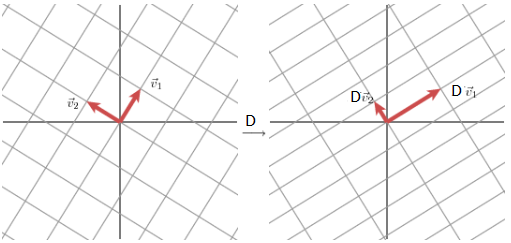
\includegraphics{SVD.png}

Es decir, los vectores $v_i$ forman una base ortonormal del espacio de salida. $D$ los agarra y devuelve otros vectores ortogonales (del espacio de llegada) posiblemente estirados. \\
A los vectores $u_i$ los formamos normalizando los vectores $D u_i$. El dibujito es este:

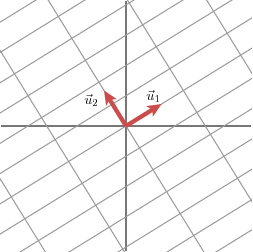
\includegraphics{SVD2.png}

(Aclaro que las imágenes fueron robadas impunemente del artículo \url{http://www.ams.org/publicoutreach/feature-column/fcarc-svd}, cuya lectura recomiendo)

Volviendo, tenemos que calcular estos vectores $u_i$ aprovechando que sabemos que $D v_i = \sigma_i u_i$. Queremos pasar dividiendo $\sigma_i$, pero NO SE PUEDE DIVIDIR POR $0$ así que tenemos que distinguir ese caso. Como están ordenados de mayor a menor, llamamos $r = \max\{i : \sigma_i > 0\}$. Este número coincide con el rango de $D$.

Si $i\leq r$ entonces $u_i = \frac{D v_i}{\sigma_i}$. Ahora bien, $v_i = e_i$ luego $u_i = \frac{col_i(D)}{\sigma_i}$. Además, $D$ era diagonal. Su i-ésima columna es justamente $d_{ii} e_i$ así que (recordando quiénes eran los $\sigma_i$) tenemos que $u_i = \frac{d_{ii} e_i}{|d_{ii}|} = sgn(d_{ii}) e_i$.

Si $i>r$ entonces completamos los $u_i$ a la base canónica. Más formalmente:

$u_i =
    \begin{cases}
        sgn(d_{ii})\ e_i  & \text{si $i\leq r$} \\
       e_i & \text{si $i>r$}
    \end{cases}$

Bien, ya tenemos una decomposición $SVD$ de $D$ (asumiendo $m \geq n$ y que los autovalores de $D$ aparecían ordenados en la diagonal).

¿Cómo conseguimos otra?

Funciona \say{pasarle los signos} de los $u_i$ a los $v_i$. Una intuición de por qué funciona, que usa un resultado útil, es la siguiente:

Vale que si $D = U\Sigma V^t$ entonces $D = \displaystyle\sum_{i=1}^n u_i \sigma_i v_i^t = \sum_{i=1}^r u_i \sigma_i v_i^t$ donde los $v_i$ y los $u_i$ son las columnas de $V$ y de $U$ respectivamente. Observemos que esto dice que estamos descomponiendo a $D$ en una suma de $r$ matrices de rango $1$ (vimos varios ejemplos en la cursada: son el resultado de multiplicar un vector columna por un vector fila). Es un lindo ejercicio para hacer (sugerencia, prueben que tanto $D$ como la expresión dan lo mismo multiplicado por una base del espacio - y usen un ejercicio de la primer práctica).

Si defino a los $u_i$ como los canónicos y $v_i$ como los vectores que tienen el signo de $d_{ii}$, la expresión de recién no cambia. En realidad esto es suficiente para demostrar que obtuvimos otra decomposición, pero se puede chequear que si definimos unas nuevas $U$ y $V$ con ese swap de signos, las cosas funcionan. Queda de ejercicio; si hacen la cuenta van a pasar por una expresión muy parecida a la de arriba.

Sin embargo, el alumno o la alumna avispada tal vez esté leyendo esto y grite \say{¡pero los $d_{ii}$ podrían ser todos positivos, o $0$! Tal vez no obtuvimos otra descomposición, man.}

Y tendría razón. Entonces una manera de asegurarnos la victoria sería multiplicar a todos los $v_i$ por $-1$ y a todos los $u_i$ por $-1$. Esto se consigue multiplicando por $-Id$ (del tamaño adecuado) a cada lado:

$D = U\Sigma V^t \Rightarrow (-Id) D (-Id) = (-Id) U \Sigma V^t (-Id)$.

La expresión de la izquierda no cambia (¡chequearlo si dudan!). Luego obtenemos: $D = \hat{U} \Sigma \hat{V^t}$, con $\hat{U} = (-Id) U, \hat{V} = (-Id) V$. Y listo. \bigskip

Mentira que listo. Faltan dos casos. Se matan rápido:

\begin{itemize}
    \item Si $m <n$ (y los autovalores están ordenados) definimos $\tilde{D} = D^t$. Esta cumple $m> n$. En particular es mayor o igual, así que por el razonamiento anterior obtenemos una descomposición SVD para la matriz: digamos que  $\tilde{D} = \tilde{U} \tilde{\Sigma} \tilde{V}^t$. Transponiendo a cada lado de la igualdad conseguimos una descomposición SVD para $D$.
    \item ¿Qué pasa si los $\sigma_i$ no están ordenados de mayor a menor? Hacemos algo parecido al primer ítem: obtenemos una matriz $\tilde{D}$ con los autovalores ordenados de mayor a menor. Esto se hace multiplicando a izquierda y a derecha por matrices de permutación apropiadas $O_1$ y $O_2$. Sabemos que existen, y no es difícil calcularlas. Digamos que $\tilde{D} := O_1 D O_2$ es la matriz diagonal con los autovalores de $D$ ordenados. Por lo argumentado (incluso si $m<n$) podemos obtener una descomposición SVD para la matriz. Nuevamente digamos que  $\tilde{D} = \tilde{U} \tilde{\Sigma} \tilde{V}^t$. Es decir, $O_1 D O_2 = \tilde{U} \tilde{\Sigma} \tilde{V}^t$. Por lo tanto $D = \underbrace{O_1^t \tilde{U}}_{U} \tilde{\Sigma} \underbrace{\tilde{V}^t O_2^t}_{V^t}$ es la descomposición que queremos.
\end{itemize}



Un par de comentarios antes de terminar el ejercicio:  

\begin{itemize}
    \item En la cuenta de recién $O_1^t \tilde{U}$ le cambia las \textit{filas} a la matriz, así que no sucede que simplemente se desordenen los $u_i$ (pasa algo parecido con los $v_i$). Es decir, no aparecen los vectores canónicos desordenados de la resolución que hicimos en el pizarrón. De todas maneras, como los vectores son los canónicos, quedan otros vectores canónicos. ¿Se podrá, definiendo otras $\tilde{D}, O_1, O_2$, forzar a que aparezcan?
    \item Al principio del ejercicio, podríamos haber calculado $D D^t$ si teníamos que $m<n$ (en vez de $D^t D)$ para arreglar el tema de los ceros. O podríamos haber calculado cualquiera y distinguir entre los dos casos a lo largo del ejercicio, o agregar notación. Hay muchas resoluciones distintas.
    \item Las matrices $O_1$ y $O_2$ se pueden calcular efectivamente. $O_1$ debe intercambiar las filas de $D$. ¿Cómo? Pues tiene que mandar el autovalor más grande a la fila $1$, el segundo autovalor más grande a la fila $2$, etc. Va a ser un producto de matrices de permutación $P_{ij}$. Una vez hecho esto, convencerse de que, como $D$ es diagonal, en realidad $O_2$ tiene que hacer un trabajo equivalente a $O_1$ pero con las columnas de $O_1 D$ (para llevar a los elementos correspondientes a la diagonal de la matriz). Es decir, resulta que $O_2 = O_1$. 
\end{itemize}




\bigskip\bigskip\bigskip\bigskip\bigskip

%Ejercicio 2: Hallar una descomposición en valores singulares de la matriz SARASA, siendo $D$ una matriz diagonal cuadrada de $n\times n$, y $e_i$ el $i$-ésimo vector canónico de $\mathbb{R}^n$. Describir explícitamente las dimensiones de las matrices $U,\Sigma$ y $V$ de su $SVD$, sus elementos, y cómo fueron calculados.


\textbf{ Ítem (b)}: Hallar una descomposici\'on en valores singulares de la matriz $\begin{pmatrix} D \\ e_i^t \end{pmatrix}$, siendo $D$ una matriz diagonal cuadrada de $n\times n$ y $e_i$ el $i$-\'esimo vector can\'onico de $\mathbb{R}^n$. Describir de forma expl\'icita las dimensiones de las matrices $U, \Sigma$ y $V$ de su SVD, sus elementos, y c\'omo fueron calculados. (12 pts.) \\


Llamemos $A$ a la matriz. Como antes, calculemos $A^t A$.

Notemos que $A^t\in \R{n}{(n+1)}, A\in\R{(n+1)}{n} \Rightarrow A^t A \in \R{n}{n}$. Además, como $D$ es diagonal y por lo tanto simétrica, $A^t = \begin{pmatrix} D\ e_i \end{pmatrix}$ así que multiplicando por bloques obtenemos que $A^t A = D^2 + e_i e_i^t$. Es decir, obtuvimos la siguiente matriz:

\iffalse
$$\begin{pmatrix}
d_{11}^2 & 0 & \cdots & 0\\
0 & d_{22}^2 & \cdots & 0\\
\cdots \\
0 & \cdots & d_{ii}^2 +1 & 0 & \cdots & 0\\
\cdots
0 & \cdots & d_{nn}^2
\end{pmatrix}$$
\fi


% que lindo que queda asi!
\[
  A^t A =
  \begin{bmatrix}
    d_{11}^2 & & \\
    & \ddots & \\
    & & d_{ii}^2 +1\\
    & & & \ddots & \\
    & & & & d_{nn}^2
  \end{bmatrix}
\]


Esta matriz es diagonal, así que tiene los autovalores bien a la vista. Nuevamente los elementos de la diagonal pueden no venir de mayor a menor. Esta vez usemos otro \say{approach}: Sea $\sigma_1$ la raíz cuadrada del autovalor más grande y $\hat{e}_1$ el vector canónico asociado a ese autovalor (si hay autovalores repetidos, elegimos alguno), $\sigma_2$ la raíz cuadrada del segundo autovalor más grande, $\hat{e}_2$ el asociado a ese autovalor, y así siguiendo hasta $\sigma_n, \hat{e}_n$.

Sea $r$ el rango de $A$, que coincide con la cantidad de valores singulares (elementos de la diagonal de $A^t A$ que son distintos de cero).

Como $A v_j = \sigma_j u_j$, si $j \leq r$ podemos pasar dividiendo y definimos $u_j = \frac{A v_j}{\sigma_j}$. Ojo, usamos el índice $j$ porque $i$ ya está tomado en el enunciado.

Como $v_j = \hat{e}_j$, tenemos que si $j\leq r$ entonces $u_j$ es una columna de $A$ dividida por $\sigma_j$.

Tenemos que inventarnos alguna notación para el número de columna. Una manera es decir que $\hat{e}_j = e_{f(j)}$, con $f$ un simple reordenamiento del conjunto $\{1,\cdots, n\}$ (otra manera de verlo es que $f$ es una función biyectiva). Es como si les pasáramos los sombreros a los índices.

Hagamos eso. Entonces $u_j = \frac{A e_{f(j)}}{\sigma_j}$ = $\frac{col_{f(j)}(A)}{\sigma_j}$. Ojo que el $e_{f(j)}$ que aparece pertenece a $\mathbb{R}^n$.

$\sigma_j$ era el $j$-ésimo de los autovalores de $A^t A$ ordenados de mayor a menor (y ese ordenamiento estaba dado por la función $f$ que definimos).

Hay uno de los $\sigma_j$ que es especial: el que es $\sqrt{d_{ii}^2+1}$. Es más, es el que tiene $j= f^{-1}(i)$ (¡a meditarlo!).

Si $j \neq f^{-1}(i)$ entonces $u_j = \frac{d_{f(j)f(j)} e_{f(j)}}{\sigma_j} = \frac{d_{f(j)f(j)} e_{f(j)}}{|d_{f(j)f(j)}|} = sgn(d_{f(j) f(j)}) e_{f(j)}$. Como el $e_{f(j)}$ que aparece provino de la multiplicación por la matriz $A$, pertenece a $\mathbb{R}^{n+1}$.


Si $j= f^{-1}(i)$, entonces $u_j = \frac{d_{f(j)f(j)} }{\sqrt{d_{f(j)f(j)}^2+1}} e_{f(j)}$. No es tan feo, solo que no se cancelan cosas.


Recordemos que todo esto era si $i \leq r$ (el rango de la matriz). Si $i>r$ entonces tenemos que completar los $u_i$ a una base ortogonal de $\mathbb{R}^{n+1}$. ¿Cómo? Con los vectores de la base canónica que faltan.

Conseguidos los $u_j$, los $\sigma_j$, y los $v_j$, obtenemos la descomposición SVD de la matriz en $U \Sigma V^t$. Con un razonamiento idéntico al del ejercicio $1$ con $m=n+1$ (y chequeando que los tamaños de los vectores que conseguimos hayan sido los correctos), tenemos que $U\in \R{(n+1)}{(n+1)}, \Sigma \in \R{(n+1)}{n}, V \in \R{n}{n}$. \bigskip


%Nota: hay algoritmos para actualizar la descomposición $SVD$ de una matriz cuando le agregamos una fila, así que si sabemos hacer eso entonces otra manera de encarar el ejercicio es usando el ítem $a$, pero en este caso es más fácil computar la $SVD$ directamente.
\end{document}